\ntextbox{Newton-Raphson's Method for Locating Roots}{
    If you have taken an introductory course in calculus you may remember the Newton-Raphson method for finding roots (zero-crossings) of functions.  The general idea behind the method locates a root by taking steps progressively closer to the unknown point starting from an initial guess.  Following a summary of the method below, we'll extend the method to solve inverse problems.

    Take a continuous and differentiable function $y = f(x)$.  Unless the initial guess is sitting at a minimum or maximum, a line drawn tangent to the initial point at $(x_i, f(x_i))$ must intersect a horizontal line running through the root\footnote{The method you may have learned is based on points which sit on the $x$-axis.  I will take a slightly more general approach here, allowing for a root at any arbitrary $y = d$, and hence the horizontal line intersected by the tangent is parallel to the $x$-axis.} (Figure~\ref{fig:nrinv}).  The equation the tangent line can be given by
    \[
        y - f(x_i) = f'(x_i)(x - x_i) ,
    \]
    where $f'(x_i)$ is the slope of the tangent line (derivative of $f(x)$ at $x = x_i$).  The value of $x$ is at this point unknown until we select the value at $y$ that we wish to know the value of $x$.  Suppose we collected data and found $y = d$.  The intersection of our tangent line above and $y = d$ is then said to occur at $x_{i+1}$ and
    \[
        d - f(x_i) = f'(x_i)(x_{i+1} - x_i) .
    \]
    Solving for $x_{i+1}$, we find
    \begin{equation}
        x_{i+1} = x_i + \frac{d - f(x_i)}{f'(x_i)} .
        \label{eq:newtraph}
    \end{equation}
    We can define our misfit then as
    \begin{equation}
        \phi = (d - f(x_{i+1}))^2 .
    \end{equation}
    If our misfit is below our desired precision, then we assume $x_{i+1} \approx x_{\text{true}}$, where $x_{\text{true}}$ is the location of the root.  If not, then we repeat Equation~\ref{eq:newtraph} with a tangent line through $f(x_{i+1})$ and so forth until our misfit falls below the desired precision (or converges, asymptotically approaches some small value).
    \begin{center}
        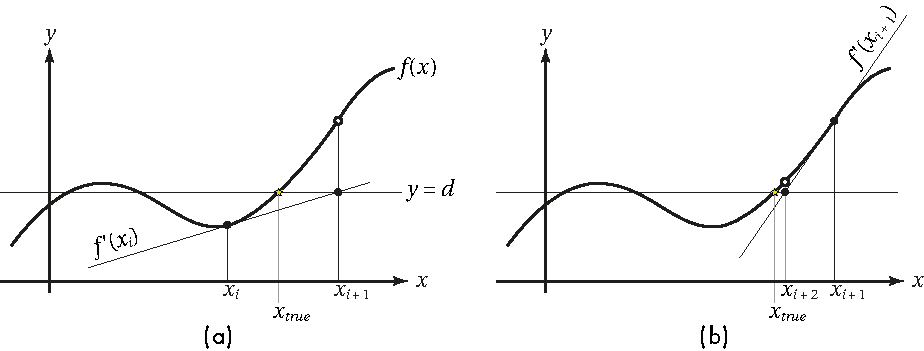
\includegraphics[]{numerical/figures/newton_raphson.eps}\\
        \textbf{Figure~\thefigure:} An illustration of the Newton-Raphson method for finding roots, generalized to an arbitrary value of a function ($y = d$).  One step (a) leads to the next (b), closer to the unknown point $x_{\text{true}}$ where the function $y = f(x)$ intersects $y = d$.  The point determined by the Newton-Raphson method can be dependent upon the initial guess.  This can be predicted using this example by imagining a starting point on the opposite side of the minimum as $x_i$.
        \label{fig:nrinv}
    \end{center}

    One more comment on Newton-Raphson's method before we move on because it illustrates an important point with respect to inversions in general.  Where there are multiple crossings at the desired level of the function (e.g., $y = d$ as in Figure~\ref{fig:nrinv}), the location of the starting point will affect which point the solution converges towards.  Put the starting point on the opposite side of the minimum in Figure~\ref{fig:nrinv} and you can by eye or by hand see that a different intersection point will be identified.  This shows why our we need to be mindful of our initial condition to our iterative inversion schemes.
}{mathtool}\label{box:newton_raphson}